\newpage
\section {Creating and using Stored Procedures:}
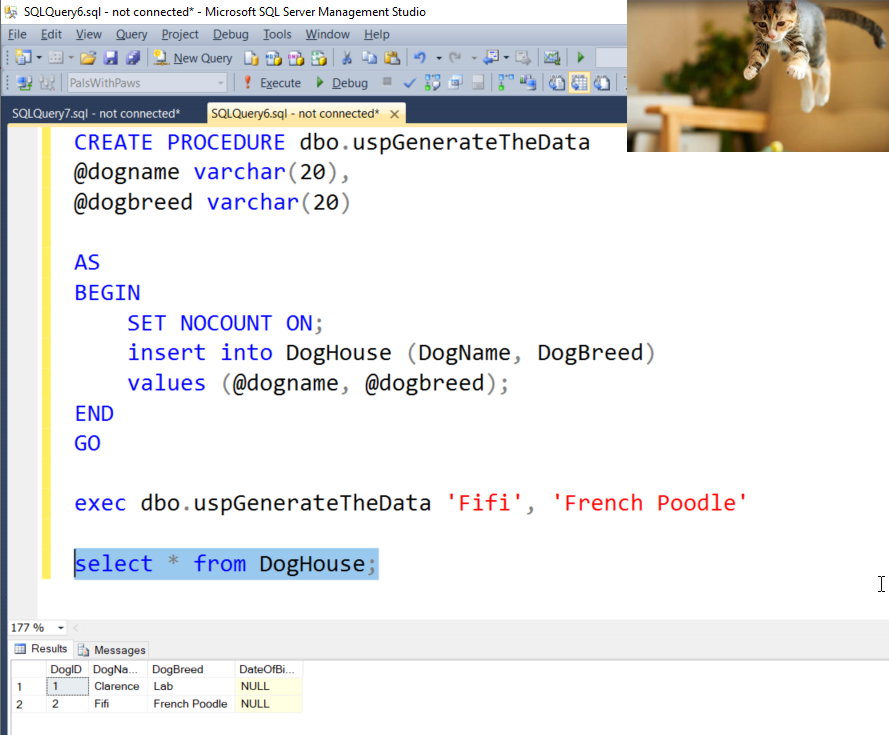
\includegraphics[]{images/Running Stored Procedures.png}
\subsection {What is a Stored Procedure?}

\subsection{Why do we use Stored Procedures?}
\begin{itemize}
    \item S.P. can be called by outside program (eg JavaScript)
    \item S.P. can called by a a TRIGGER (which is just any condition in the database
    such as a certain table going above 1000 rows in number of records).
    \item Stored Procedures can provide a LIBRARY of Routines to make our development
    work speedier, less tiring, more efficient.
\end{itemize}

\subsection{How do we use Stored Procedures?}

\emph{Create a Stored Procedure:}
\begin{Verbatim}[frame=single]
create database PalsWithPaws;
GO

    CREATE PROCEDURE GenerateTheTables
    
    AS
    BEGIN
    	SET NOCOUNT ON;
    	create table DogHouse(
    		-- this is a comment
    		-- note how we set an AUTOINCREMENTING prmary key!
    		DogID int IDENTITY(1,1) PRIMARY KEY,
    		DogName varchar(20) not null,
    		DogBreed varchar(20) not null,
    		DateOfBirth datetime2 
    	);
    END
    GO
\end{Verbatim}

\emph{RUN a Stored Procedure:}
\begin{Verbatim}[frame=single]
exec GenerateTheTables
\end{Verbatim}

\section * {Parameterizing queries}
One of the benefits of SQL is the ability to write a query and use parameters to dynamically act upon the resultset. Depending on the situation, there can be benefits to parameterizing queries, but it is not always clear when or how to do this.  In this tip we look at different ways to pass in values as parameters to queries and the advantages and disadvantages.

\begin{Verbatim}[frame=single]

CREATE PROCEDURE dbo.uspGenerateTheData
@dogname varchar(20),
@dogbreed varchar(20)

AS
BEGIN
	SET NOCOUNT ON;
	insert into DogHouse (DogName, DogBreed) 
	values (@dogname, @dogbreed);
END
GO

\end{Verbatim}


